%%%%%%%%%%%%%%%%%%%%%%%%%%%%%%%%%%%%%%%%%%%%%%%%%%%%%%%%%% 
\chapter{はじめに} \label{chap:intro}
\pagenumbering{arabic}
%%%%%%%%%%%%%%%%%%%%%%%%%%%%%%%%%%%%%%%%%%%%%%%%%%%%%%%%%% 

電力網の構成制御は,エネルギーの節約や安定した電力供給を支える重要な研
究課題である\cite{25627,103687}.
電力網は,高電圧で発電所と変電所を結ぶ\textbf{送電網}と,
低電圧で変電所と家庭や工場といった需要家を結ぶ\textbf{配電網}に分類される.
配電網は変電所と需要家との間で構成される電力供給ネットワークであり,そ
の構成技術はスマートグリッドや,災害時の障害箇所の迂回構成などを支える
重要な基盤技術である.

\textbf{配電網問題}は,
供給経路に関する\textbf{トポロジ制約}と,
電流・電圧に関する\textbf{電気制約}を満たしつつ,
電力の損失を最小にするスイッチの開閉状態を求めることが目的である~\cite{Hayashi:dnet:model}.
トポロジ制約は,
短絡(供給経路上のループ,複数の変電所と結ばれる需要家)と
停電(変電所と結ばれない需要家)が発生しないことを保証する.
電気制約は,
供給経路の各区間で許容電流を超えないこと,
電気抵抗による電圧降下が許容範囲を超えないことを保証する.

%%%%%%%%%%%%%%%%%%%%%%%%%%%%%%%
\begin{figure}[tbp]
 \centering
 %%%%%%%%%%%%%%%%%%%%%%%%%%%%%%%%%%%%%%%%%%%%%%%%%%
% 配電網 例 (第1章で使う)
%%%%%%%%%%%%%%%%%%%%%%%%%%%%%%%%%%%%%%%%%%%%%%%%%%

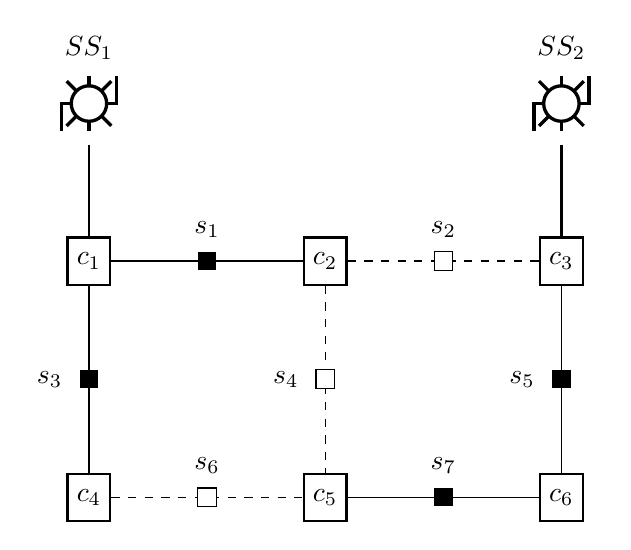
\begin{tikzpicture}

 % 設定
 \tikzset{customer/.style={rectangle,thick,draw=black,minimum height=0.6cm}}
 \tikzset{on_switch/.style={rectangle,fill=black}}
 \tikzset{off_switch/.style={rectangle,draw=black,fill=white}}

 % 補助線
 % \draw [help lines,blue,step=1cm] (-5,0) grid (5,-5);
  
 % substation1 (ホントはnewcommandでできるようにしたかった...)
 \draw [very thick] (-3,0) circle [radius=0.225cm] node[draw=white,minimum size=1cm](root1){};
 \draw [very thick] (-2.775,0)--(-2.65,0)--(-2.65,0.35);
 \draw [very thick] (-3.225,0)--(-3.35,0)--(-3.35,-0.35);
 \draw [very thick] (-3,0.225)--(-3,0.35);
 \draw [very thick] (-3,-0.225)--(-3,-0.35);
 \draw [very thick] [domain=-0.284:-0.159] plot(\x-3,\x);
 \draw [very thick] [domain=0.159:0.284] plot(\x-3,\x);
 \draw [very thick] [domain=-0.284:-0.159] plot(\x-3,-\x);
 \draw [very thick] [domain=0.159:0.284] plot(\x-3,-\x);
 \node at (-3,0.7) {$SS_{1}$};

 % substation2
 \draw [very thick] (3,0) circle [radius=0.225cm] node[draw=white,minimum size=1cm](root2){};
 \draw [very thick] (3.225,0)--(3.35,0)--(3.35,0.35);
 \draw [very thick] (2.775,0)--(2.65,0)--(2.65,-0.35);
 \draw [very thick] (3,0.225)--(3,0.35);
 \draw [very thick] (3,-0.225)--(3,-0.35);
 \draw [very thick] [domain=-0.284:-0.159] plot(\x+3,\x);
 \draw [very thick] [domain=0.159:0.284] plot(\x+3,\x);
 \draw [very thick] [domain=-0.284:-0.159] plot(\x+3,-\x);
 \draw [very thick] [domain=0.159:0.284] plot(\x+3,-\x);
 \node at (3,0.7) {$SS_{2}$};

 % 需要家 customer
 \node[customer] at (-3,-2)(1){$c_1$};
 \node[customer] at (0,-2) (2){$c_2$};
 \node[customer] at (3,-2) (3){$c_3$};
 \node[customer] at (-3,-5) (4){$c_4$};
 \node[customer] at (0,-5) (5){$c_5$};
 \node[customer] at (3,-5) (6){$c_6$};

 % 辺
 % ルート
 \draw [thick] (root1) -- (1);
 \draw [thick] (root2) -- (3);
 % 繋がってない辺は点線
 \foreach \u / \v in {2/3, 2/5, 4/5}
 \draw [dashed] (\u) -- (\v);
 % 繋がってる辺は実線
 \foreach \u / \v in {1/2, 1/4, 3/6, 5/6}
 \draw (\u) -- (\v);

 % スイッチ switch %
 % \node[on_switch] at (-3,-1) (s1){};
 % \node at (-3.5,-1) {$s_1$};
 %
 % \node[on_switch] at (3,-1) (s2){};
 % \node at (2.5,-1) {$s_2$};
 %
 \node[on_switch] at (-1.5,-2) (s1){};
 \node at (-1.5,-1.6) {$s_1$};
 %
 \node[off_switch] at (1.5,-2) (s2){};
 \node at (1.5,-1.6) {$s_2$};
 %
 \node[on_switch] at (-3,-3.5) (s3){};
 \node at (-3.5,-3.5) {$s_3$};
 %
 \node[off_switch] at (0,-3.5) (s4){};
 \node at (-0.5,-3.5) {$s_4$};
 %
 \node[on_switch] at (3,-3.5) (s5){};
 \node at (2.5,-3.5) {$s_5$};
 %
 \node[off_switch] at (-1.5,-5) (s6){};
 \node at (-1.5,-4.6) {$s_6$};
 %
 \node[on_switch] at (1.5,-5) (s7){};
 \node at (1.5,-4.6) {$s_7$};
 %

\end{tikzpicture}

%%%%%%%%%%%%%%%%%%%%%%%%%%%%%%%%%%%%%%%%%%%%%%%%%%%%%%%%%%
%%% Local Variables:
%%% mode: japanese-latex
%%% TeX-master: paper.tex
%%% End:

 \caption{配電網問題の例}
 \label{fig:dnet}
\end{figure}
%%%%%%%%%%%%%%%%%%%%%%%%%%%%%%%

トポロジ制約のみの配電網問題の例を図\ref{fig:dnet}に示す.
この例は,
2つの変電所$\{SS_{1}, SS_{2}\}$,
7個のスイッチ$\{s_{1},\ldots, s_{7}\}$,
6つの需要家$\{c_{1},\ldots, c_{6}\}$から構成されている.
$\blacksquare$は閉じたスイッチ,
$\square$は開いたスイッチを表している.
配電網問題の実行可能解は閉じたスイッチの集合で表すことができる.
この例は実行可能解$\{s_{1},s_{3},s_{5},s_{7}\}$を表している.
需要家$\{c_{1},c_{2},c_{4}\}$は変電所$SS_{1}$から,
需要家$\{c_{3},c_{5},c_{6}\}$は変電所$SS_{2}$から電力を供給され,
トポロジ制約を満たしていることがわかる.

配電網問題は求解困難な組合せ最適化問題の一種であり,
これまでフロンティア法を用いた解法等が提案されている~\cite{Minato:dnet:ZDD}.
% 井上さんのtheory.pdfもbibtex作ってここに入れる
本研究ではトポロジ制約のみの配電網問題を対象とする.
トポロジ制約のみの配電網問題は,
与えられた連結グラフと根と呼ばれる特殊なノードから,
\textbf{根付き全域森}を求める部分グラフ探索問題に
帰着できることが知られている.
以降,この問題を\textbf{根付き全域森探索問題}
(Spanning Rooted Forest Problem; SRFP)と呼ぶ.

\textbf{解集合プログラミング}(Answer Set Programing; ASP\cite{%
  Baral03:cambridge,%
  Gelfond88:iclp,%
  Niemela99:amai,%
  Inoue08:jssst})は,
論理プログラミングから派生したプログラミングパラダイムである.
ASP言語は,一階論理に基づく知識表現言語の一種であり,論理プログラムは
ASPのルールの有限集合である.
ASPシステムは論理プログラムから安定モデル意味論\cite{Gelfond88:iclp}
に基づく解集合を計算するシステムである.
近年,SATソルバーの技術を応用した高速なASPシステムが確立され,制約充足問題,
プランニング,システム生物学,時間割問題,システム検証など様々な分野への
実用的応用が急速に拡大している\cite{ASPAISAT}.

% プログラムの名前を dnet -> srf に変更 (解いてるのSRFなので...)
本論文では,解集合プログラミング(ASP)を用いた根付き全域森探索問題
(SRFP)の解法について述べる.
まず,根付き全域森探索問題を解く2種類のASP符号化
\code{srf1}と\code{srf2}を考案した.
これらの符号化は,SRFPの制約を7つまたは6つのASPのルールで
簡潔に表現している.
\code{srf1}符号化は,SRFPの根付き連結制約を
at-least-one制約とat-most-one制約で表現した基本的な符号化に対し,
\code{srf2}符号化は,根付き連結制約をASPの個数制約を用いて表現している点が
特長である.
\code{srf2}符号化は,\code{srf1}符号化と比較すると基礎化後の制約数を
少なく抑えることができるため,大規模な問題に対する有効性が期待できる.

また,障害時の復旧予測への応用を狙いとした,
ある初期配電網の構成からスタートして,
トポロジ制約を満たした上で,一度に切り替えるスイッチの数を$k$個以下に制限し,
最終的に目的とする配電網の構成を得るためのスイッチの切り替え手順を求め
る遷移問題への拡張も行った.

考案した符号化の有効性を評価するために,
DNET (Power Distribution Network Evaluation Tool)~\footnote{%
\url{https://github.com/takemaru/dnet}}
に公開されている問題(3問)と,
Graph Coloring and its Generalizations~\footnote{%
\url{https://mat.tepper.cmu.edu/COLOR04/}}
に公開されているグラフ問題を元に生成した問題(82問)を用いて,
実行実験を行なった.
その結果,
\code{srf2}符号化は,\code{srf1}符号化より多くの問題を
解くことに成功した.
また,\code{srf2}符号化はスイッチ数が40,000個を超えるような大規模な問
題も解いており,配電網問題に対する ASP の有効性が確認できた.

本論文の構成は,
第\ref{chap:dnet}章で根付き全域森の定義を示し,
第\ref{chap:asp}章で解集合プログラミングの説明を行う.
第\ref{chap:prop}章で根付き全域森問題のASP符号化と考案したプログラムを示し,
第\ref{chap:exp}章で考案したプログラムの評価実験とその考察を述べる.
第\ref{chap:trans}章で根付き全域森問題の遷移問題への拡張を行い,
第\ref{chap:conc}章で本稿についてまとめる.


%%% Local Variables:
%%% mode: japanese-latex
%%% TeX-master: "paper"
%%% End:
